As described earlier, graphical modeling languages and transformations bind together functions of the toolchains.  These languages are defined using metamodels in the Generic Modeling Environment (GME) \cite{isis:gme}, which is also used directly to edit models thus represented.  Graph transformations are specified using GReAT \cite{isis:great}.  These generic tools aim to provide the necessary framework to enable an end-to-end development solution: from functional design using Simulink/Stateflow, through verification of critical operational properties, down to certified code that can be used confidently on the specified platform.  Here we describe details of the modeling languages in the tools and the intended design flow.

In a typical design, a control designer will capture physical models mathematically, and then represent them in a simulation tool such as Simulink.   Controllers are then specified by adding dataflow model elements to the Simulink model, possibly with state-based controller elements specified in Stateflow. Implementations of the controller functions may be generated in C code using Real-Time workshop, or written by hand.  Next, the implementation must be pasted into a software design framework, which was likely created using UML tools.  Testing and debugging follow, then  final deployment.

Envision instead a tool that imports Simulink and Stateflow models directly into a model-based software design environment.  Within this environment are additional modeling languages that describe software component partitions and interfaces, as well as hardware descriptions.   ECSL-DP (Embedded Control System Language for Distributed Processing) is an aggregate language that includes all of these constructs \cite{KS:ISIS-04-505}. Figure \ref{fig:packages} depicts the elements of the language.  The components, platform, and mapping languages of ECSL-DP will be described here, with highlights of important constructs.

\begin{figure}[h]
\begin{center}
   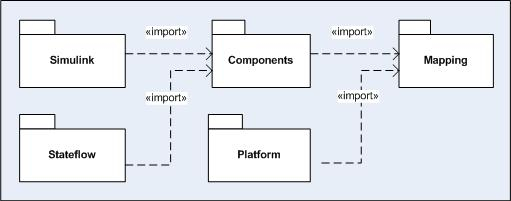
\includegraphics[width=0.9\columnwidth]{packages}
   \caption{Relationships between sublanguages in ECSL-DP.}
   \label{fig:packages}
\end{center}
\end{figure}

\begin{figure}[h]
\begin{center}
   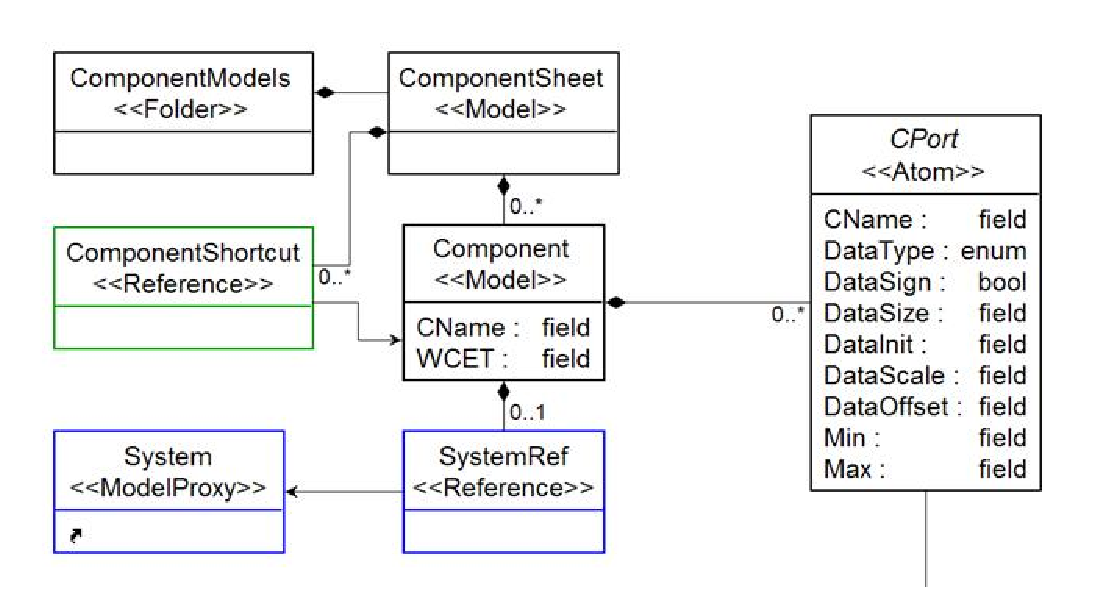
\includegraphics[width=0.9\columnwidth]{component_meta}
   \caption{Fundamental elements of component models in ECSL-DP.}
   \label{fig:CompMeta}
\end{center}
\end{figure}

Figure \ref{fig:CompMeta} illustrates the basic elements of the modeling language for describing the allocation of Simulink blocks to software components.   Components refer to Simulink Systems, and have ports (interfaces) for exchanging data.  The meta-programmable modeling environment allows us to extend the language with particular concepts, such as real-time execution time constraints as shown in Figure \ref{fig:RealTime}.  This modeling construct is not currently used by the code generators, but illustrates the extension mechanism for adding future capabilities.

\begin{figure}[h]
\begin{center}
   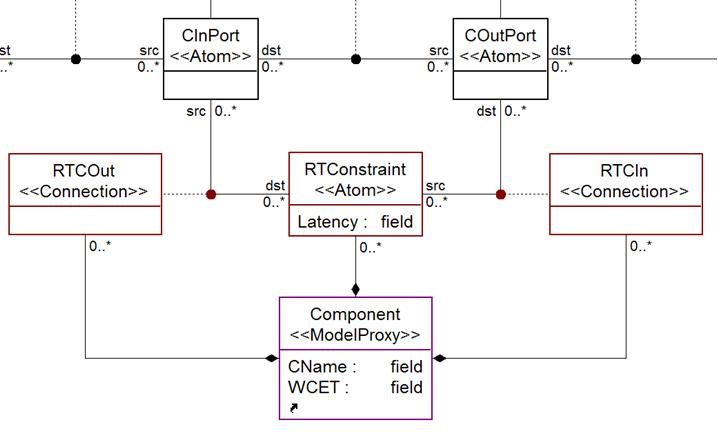
\includegraphics[width=0.9\columnwidth]{real_time}
   \caption{Real-time execution constraint models for components in ECSL-DP.}
   \label{fig:RealTime}
\end{center}
\end{figure}

The key parts of ECSL-DP provide the most benefit over alternative code-generation schemes.  In ECSL-DP hardware platforms are modeled directly, and then the component architecture is mapped onto the hardware topology using graphical modeling tools.   Hardware models are simple networks of processing elements and communication buses.  Model parameters include data transfer rates and other essential configuration items.  Figure \ref{fig:MappingMeta} shows metamodel elements for this mapping.  The modeling languages for platforms and components are composed to form a new sublanguage within ECSL-DP, which precisely defines the relationship between concepts in both languages.  Software components are assigned to tasks, which are assigned to run on a single processing element.  Tasks specify the period of cyclic execution.  The mapping also defines communication messages for connected buses, and relates them to communication ports in the component model.

\begin{figure}[h]
\begin{center}
   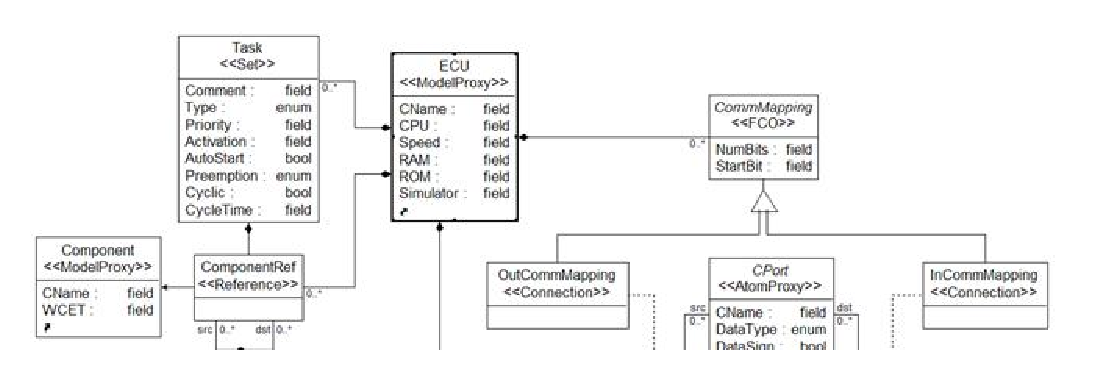
\includegraphics[width=0.9\columnwidth]{mapping_meta}
   \caption{Metamodel for mapping software components to platform elements.}
   \label{fig:MappingMeta}
\end{center}
\end{figure}
     
     In summary, consider the different aspects of the model:  Start with functional blocks connected by signals; These are wrapped, respectively, into components and their associated communication channels, which are mapped (respectively) to tasks on processors and messages on buses.  The resulting layered model captures all of the necessary information to generate code, create time-triggered schedules, and configure the platform.  These functions are currently available in the toolchain, and they are implemented using model interpreters and graph transformations, described below.  The next steps in tool evolution will add verification concepts at different stages of the design and integrate the proper tools to enable safety-assured software designs.
